%!TEX root = main.tex
\section{Background}

La hoja de estilo está diseñada de forma que se pueden usar las etiquetas
habituales de la hoja de estilo {\tt article}, introduciendo sólo unas pequeñas
modificaciones. Sugerimos a los autores que tomen el fichero {\tt ejemplo.tex}
con el que se ha generado este documento, como plantilla para sus propios
trabajos, conservando en todo lo posible las definiciones, márgenes y
declaraciones que definen tanto la Hoja de Estilo como la propia plantilla. Una
buena idea es comprobar el efecto que tienen las distintas órdenes incluidas en
el fichero fuente de \LaTeX{} ({\tt ejemplo.tex}) sobre la apariencia final del
documento en formato PDF ({\tt ejemplo.pdf}).

Primero, para seleccionar la hoja de estilo se debe escribir la siguiente orden
\begin{center}
\verb+\documentclass[twocolumn,twoside]{Jornadas}+
\end{center}

Esta hoja de estilo no permite incluir las filiaciones de los autores justo
debajo de sus nombres. Esta información se incluirá en notas al pie de la
primera página mediante el uso de la orden \verb+\thanks{...}+. Tal y como puede
verse en este documento de ejemplo, se ha asociado una orden a cada uno de los
autores. Esto da lugar a la inclusión de una nota al pie por cada uno de ellos.
Los agradecimientos a proyectos deben incluirse en la sección final del
artículo.

El primer párrafo del artículo debe iniciarse con la orden
``\verb+\PARstart{X}{YYY} ZZZ+''. Esta orden produce una letra grande \verb+X+
al principio de un párrafo. La cadena \verb+YYY+ se cambiará automáticamente a
letras mayúsculas.

La hoja de estilo de bibliografía {\tt Jornadas.bst} permite que el programa
\BibTeX\ incluya las referencias bibliográficas de acuerdo con el formato usado
en las actas.

En la figura~\ref{fig:programa} podemos ver la estructura de definición de un
artículo usando la hoja de estilo {\tt Jornadas.cls}. 
 
Los artículos sometidos a las Jornadas no deben contener ni cabeceras ni números
de página. Ambos elementos serán incluidos por la organización durante el
proceso de generación de las actas completas. Las órdenes \verb+\markboth{}{}+,
\verb+\pagestyle{empty}+ y \verb+\thispagestyle{empty}+ han sido añadidas al
ejemplo para ocultar tanto las cabeceras como los números de todas las páginas. 

Los comentarios de las tablas deben definirse encima de las mismas, mientras que
los comentarios de las figuras se deben colocar debajo.

\begin{figure}[htb] 
\begin{center} 
  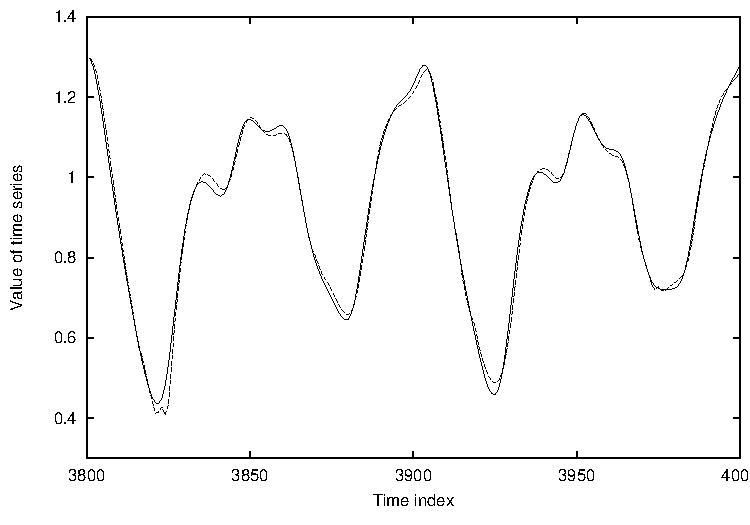
\includegraphics[width=7.5cm]{figura.pdf}
\end{center} 
\caption{Los comentarios de las figuras van debajo.} 
\label{fig:curva} 
\end{figure} 

Si quieres poner varias sub-figuras dentro de una misma figura, puedes usar el
paquete \verb+subfig+, como en la Fig.\ref{fig:subfig} (incluye Figs.~\ref{subfig:a} y \ref{subfig:b}).

\begin{figure}[ht]
    \centering
    \subfloat[Logo Sarteco]{\label{subfig:a}
    \includegraphics[width=0.4\linewidth]{Sarteco}%
    }
    \hfill
    \subfloat[Logo Jornadas]{\label{subfig:b}
    
\includegraphics[width=0.4\linewidth]{Jornadas}%
    }
    \caption{Algunos logos.}
    \label{fig:subfig}
    \end{figure}

\begin{table}[htb]
\caption{Ejemplo de tabla. El comentario se sitúa al comienzo de la
definición de la tabla.}
\begin{center}
{\footnotesize
\begin{tabular}{|c||c|c|}\hline
N. Proc. & t  & e   \\\hline\hline
10       & 50 & 0.5 \\\hline
20       & 25 & 0.7 \\\hline
\end{tabular}
}
\end{center}
\end{table}

Incluya sus figuras preferiblemente usando ficheros en formato {\tt .pdf} en
blanco y negro o tonos de gris (el fondo debe ser siempre blanco). 

\begin{figure*}[!t]
    \centering
    \begin{minipage}{0.9\linewidth}
    {\footnotesize
    \begin{lstlisting}[language=Python]
def XCM2(events):
    n_events = len(events) (*@\label{lin:xcm-a}@*)

    Corr_max = zeros((n_events,n_events))
    Lag_max = zeros((n_events,n_events))
    Corr_min = zeros((n_events,n_events))
    Lag_min = zeros((n_events,n_events))(*@\label{lin:xcm-b}@*)

    for i in range(n_events):(*@\label{lin:xcm-i}@*)
        for j in range(i, n_events):
            xcorrij = xcorr(events[i], events[j], 250, full_xcorr=True) (*@\label{lin:xcm-c}@*)
            #Returns index and CC[i] for max(abs(CC[i])) --including negative values--
            Lag_min[i,j] = xcorrij[0](*@\label{lin:xcm-d}@*)
            Corr_min[i,j] = xcorrij[1]
            if xcorrij[1]<0.:
                #Return highest positive CC[i] and index (xcorrij[2] contains CC)
                Lag_max[i,j], Corr_max[i,j] = xcorr_max(xcorrij[2],abs_max=False)
            else:
                Lag_max[i,j] = xcorrij[0]
                Corr_max[i,j] = xcorrij[1](*@\label{lin:xcm-e}@*)

    return Corr_max, Lag_max, Corr_min, Lag_min
    \end{lstlisting}
    }
    \end{minipage}
    \caption{Código de ejemplo en python.}
    \label{fig:originalCode}
    \end{figure*}

En la Figura~\ref{fig:originalCode} se muestra un ejemplo de uso de \verb+\lstlisting+ para insertar un bloque de código. En este ejemplo el código es Python, pero se puede cambiar el ``Syntax Highlighting'' cambiando el argumento \verb+language+, por ejemplo \verb+[language=C]+. Puedes hacer referencia a las líneas de código etiquetadas con \verb+(*@\label{lin:tu-etiqueta}@*)+, como por ejemplo las líneas~\ref{lin:xcm-a}-\ref{lin:xcm-b} del código.



